\documentclass[t,aspectratio=169,10pt]{beamer}

\usepackage[utf8]{inputenc}

\usepackage{multicol}
\usepackage{multirow}
\usepackage[absolute,overlay]{textpos}
\usepackage{tcolorbox}
\usepackage{tikz}

\usepackage{graphicx}
\graphicspath{{./figuras/}}


\title{Clase 30}
\subtitle{Escalamiento de MOSFETs}
\author{Dr.-Ing. Juan José Montero-Rodríguez}
\institute{Escuela de Ingeniería Electrónica}
\date{Semestre II-2023}
\titlegraphic{\includegraphics[height=8mm]{logoTEC.png}}


\begin{document}

\begin{frame}
\titlepage
\end{frame}


\begin{frame}
\frametitle{El Primer Transistor}

\begin{columns}

\begin{column}{0.5\textwidth}

	Patente del efecto de campo: 1925 Lillienfeld
	
	\vspace{3mm}
	Patente del MOSFET: 1928 Lillienfeld
	
	\vspace{3mm}
	Problema de fabricación del MOSFET: calidad del aislante
 
\end{column}

\begin{column}{0.5\textwidth}

	\includegraphics[width=\textwidth]{first-transistor}
	
	1947 Bardeen, Brattain, Schockley
	
	1956: Premio Nobel
 
\end{column}

\end{columns}

\end{frame}


\begin{frame}
\frametitle{El Primer Circuito Integrado}

\centering
Tecnología de circuitos integrados:

inventada por Jack Kilby, de Texas Instruments en 1958

\includegraphics[width=12cm]{first-IC}
\end{frame}


\begin{frame}
\frametitle{Primer Circuito Integrado Planar}

\begin{columns}

	\begin{column}{0.5\textwidth}
 
		\centering
		\includegraphics[width=\textwidth]{first-planarIC}
  
	\end{column}
 
	\begin{column}{0.5\textwidth}
	1961
	
	2 pulgadas de diámetro
	
	4 transistores y algunas resistencias
 
\end{column}

\end{columns}

\end{frame}


\begin{frame}
\frametitle{Transistor MOSFET}
\begin{itemize}
	\item El avance del MOSFET de una generación tecnológica a la siguiente se rige por la teoría de escalamiento
\end{itemize}

\centering
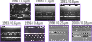
\includegraphics[width=11cm]{crosssections}

Ejemplo de escalamiento de tecnología ETOX de Intel, para memorias EEPROM
\end{frame}


\begin{frame}
\frametitle{La Revolución de la Microelectrónica}
\begin{textblock*}{7cm}(0.5cm,1.5cm)
	\raggedright
	"When you see the numbers or hear your companie's name on the evening news ... and you are once again reminded that this is \textcolor{red}{no longer an industry, but an economic and cultural phenomenon, a crucial force at the heart of the modern world"}
	
	\raggedleft (G. Moore)
\end{textblock*}

\begin{textblock*}{3.5cm}(9.5cm,1.5cm)
	\includegraphics[width=3.5cm]{revolution1}
\end{textblock*}

\begin{textblock*}{15cm}(0.5cm,5cm)
	\centering
	\includegraphics[height=3cm]{revolution2} \includegraphics[height=3cm]{revolution3} \includegraphics[height=3cm]{revolution4} \includegraphics[height=3cm]{revolution5}
\end{textblock*}

\begin{textblock*}{15cm}(0.5cm,5cm)
	\centering
	50 nm \hspace{3cm} 30 nm \hspace{3 cm} 20 nm \hspace{3cm} 15 nm
\end{textblock*}

\end{frame}


\begin{frame}
\frametitle{Ley de Moore}
\centering
"El número de transistores en un chip se duplica cada 18 meses"

\includegraphics[width=9cm]{moore}

"No exponential is forever, but 'forever' can be delayed" (G. Moore, 1965)
\end{frame}


\begin{frame}
\frametitle{Escalamiento}
\centering
\includegraphics[width=11cm]{scaling}
\end{frame}

\begin{frame}
\frametitle{Escalamiento}
\centering
\includegraphics[width=11cm]{scaling2}
\end{frame}

\begin{frame}
\frametitle{Teoría de Escalamiento}
\begin{itemize}
	\item Inicialmente propuesta por R. H. Dennard y su equipo en los 60's
	\item Las dimensiones del transistor pueden escalarse en un factor S $>$ 1, si el campo eléctrico se mantiene constante
	\item Factor de escalamiento $\approx$1.4 por generación tecnológica
\end{itemize}

\centering
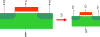
\includegraphics[width=12cm]{scaling3}

Dos tipos de escalamiento: de campo constante y de voltaje constante
\end{frame}


\begin{frame}
\frametitle{Escalamiento de Campo Constante}
\begin{itemize}
	\item Objetivo: mantener constante el campo eléctrico en el transistor y con ello, el comportamiento de un transistor de canal largo
\end{itemize}

\centering
\begin{tabular}{|c|c|c|}
	\hline \textbf{Magnitud} & \textbf{Dimensión original} & \textbf{Escalamiento} \\
	\hline Largo de canal & L & L/S \\
	\hline Ancho de canal & W & W/S \\
	\hline Espesor de óxido & t\textsubscript{OX} & t\textsubscript{OX}/S \\
	\hline Profundidad de difusión de fuente y drenador & x\textsubscript{j} & x\textsubscript{j}/S \\
	\hline Voltaje & V & V/S  \\
	\hline Concentración de dopado de substrato & N\textsubscript{A}, N\textsubscript{D} & N\textsubscript{A}*S, N\textsubscript{D}*S \\
	\hline 
\end{tabular}

\vspace{5mm}
\centering
La concentración de dopado de substrato se aumenta para escalar el ancho de la zona de agotamiento
\end{frame}


\begin{frame}
\frametitle{Escalamiento de Campo Constante}
\centering
Efectos del escalamiento de campo constante

\vspace{5mm}
\begin{tabular}{|c|c|c|}
	\hline \textbf{Magnitud} & \textbf{Valor original} & \textbf{Escalamiento} \\
	\hline Corriente de drenador & I\textsubscript{DS} & I\textsubscript{DS}/S\\
	\hline Área del transistor & A & A/S\textsuperscript{2} \\
	\hline Capacitancia de óxido & C\textsubscript{OX} & C\textsubscript{OX}/S \\
	\hline Retardo de compuerta & $\tau$ & $\tau$/S \\
	\hline Consumo de potencia & P\textsubscript{S} & P\textsubscript{S}/S\textsuperscript{2} \\
	\hline Densidad de potencia & P\textsubscript{D} & P\textsubscript{D} \\
	\hline Producto potencia-retardo & PDP & PDP/S\textsuperscript{3} \\
	\hline
\end{tabular}

\vspace{5mm}
\begin{itemize}
	\item Compuertas más rápidas
	\item Mayor densidad de integración
	\item Densidad de potencia constante
\end{itemize}
\end{frame}


\begin{frame}
\frametitle{Escalamiento de Voltaje Constante}
\begin{itemize}
	\item Objetivo: mantener constante voltaje en el transistor e intentar minimizar incrementos en el campo eléctrico
\end{itemize}

\centering
\begin{tabular}{|c|c|c|}
	\hline \textbf{Magnitud} & \textbf{Dimensión original} & \textbf{Escalamiento} \\
	\hline Largo de canal & L & L/S \\
	\hline Ancho de canal & W & W/S \\
	\hline Espesor de óxido & t\textsubscript{OX} & t\textsubscript{OX}/S \\
	\hline Profundidad de difusión de fuente y drenador & x\textsubscript{j} & x\textsubscript{j}/S \\
	\hline Voltaje & V & V  \\
	\hline Concentración de dopado de substrato & N\textsubscript{A}, N\textsubscript{D} & N\textsubscript{A}*S\textsuperscript{2}, N\textsubscript{D}*S\textsuperscript{2} \\
	\hline 
\end{tabular}

\vspace{5mm}
\centering
Se pretende mantener compatibilidad de voltajes entre generaciones tecnológicas
\end{frame}


\begin{frame}
\frametitle{Escalamiento de Voltaje Constante}
\centering
Efectos del escalamiento de voltaje constante

\vspace{5mm}
\begin{tabular}{|c|c|c|}
	\hline \textbf{Magnitud} & \textbf{Valor original} & \textbf{Escalamiento} \\
	\hline Corriente de drenador & I\textsubscript{DS} & I\textsubscript{DS}*S\\
	\hline Área del transistor & A & A/S\textsuperscript{2} \\
	\hline Capacitancia de óxido & C\textsubscript{OX} & C\textsubscript{OX}/S \\
	\hline Retardo de compuerta & $\tau$ & $\tau$/S\textsuperscript{2} \\
	\hline Consumo de potencia & P & P*S\\
	\hline Densidad de potencia & P\textsubscript{D} & P\textsubscript{D}*S\textsuperscript{3} \\
	\hline
\end{tabular}

\vspace{5mm}
\begin{itemize}
	\item Compuertas más rápidas
	\item Mayor densidad de integración
	\item Densidad de potencia aumenta $\Rightarrow$ problemas de disipación de calor
\end{itemize}
\end{frame}


\begin{frame}
\frametitle{Efectos del Escalamiento}
\begin{itemize}
	\item Voltaje de umbral escala
	\item Pendiente de subumbral $\approx$ constante
	\begin{itemize}
		\item $\Rightarrow$ Aumento de corriente de subumbral $\Rightarrow$ V\textsubscript{TH} debe ajustarse para mantenerla aproximadamente constante
	\end{itemize}
	\item Reducción de voltaje de alimentación
	\begin{itemize}
		\item Ajuste de V\textsubscript{TH} $\Rightarrow$ disminuye el voltaje efectivo V\textsubscript{GS} -V\textsubscript{TH}
		\item Debe elegirse entre alto desempeño y mayor corriente de subumbral o entre menor desempeño y menor corriente de subumbral
	\end{itemize}
	\item Compuertas más rápidas, mayor densidad de integración
	\item Densidad de potencia aumenta $\Rightarrow$ problemas de disipación de calor
	\item Efectos de canal corto
	\item Aumento en corrientes de fuga de compuerta ($V_{TH}$, $t_{OX}$)
	\item Degradación por inyección de portadores de carga calientes
\end{itemize}
\end{frame}


\begin{frame}
\frametitle{Frecuencia de Operación}
\centering
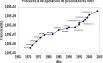
\includegraphics[width=11cm]{freqop}
\end{frame}


\begin{frame}
\frametitle{Consumo de Potencia}
\centering
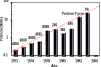
\includegraphics[width=11cm]{power}
\end{frame}


\begin{frame}
\frametitle{Consumo de Potencia de Procesadores}
\centering
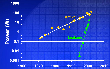
\includegraphics[width=11cm]{power2}
\end{frame}


\begin{frame}
\frametitle{Densidad de Potencia}
\centering
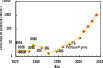
\includegraphics[width=11cm]{power3}
\end{frame}


\begin{frame}
\frametitle{Consecuencias del Escalamiento}
\begin{itemize}
	\item El escalamiento del MOSFET causa efectos que desvían su comportamiento del MOSFET de canal largo, entre los que están
	\begin{itemize}
		\item Efecto de canal corto (short channel effect)
		\item Perforación de canal (Punch-through)
		\item Degradación por portadores de carga calientes (hot carrier degradation)
	\end{itemize}
	\item Otros problemas
	\begin{itemize}
		\item Fuga de compuerta (gate leakage)
		\item Electromigración
	\end{itemize}
\end{itemize}
\end{frame}


\begin{frame}
\frametitle{Efecto de Canal Corto}

\begin{columns}

	\begin{column}{0.5\textwidth}
 
		\begin{itemize}
			\item Canal corto: la distancia entre S y D es comparable a la profundidad de la zona de agotamiento
			\item Al acortarse el canal, el campo eléctrico del drenador contribuye significativamente al agotamiento del canal
		\end{itemize}
		
		$\Rightarrow$ El canal se forma a tensiones menores que la tensión de umbral de un MOSFET de canal largo
		
		\[ V_{TH\_SC} = V_{TH\_LC} - \Delta V_{TH} \]
		
		\vspace{4mm}
		$V_{TH\_SC}$: $V_{TH}$ de canal corto
		
		$V_{TH\_LC}$: $V_{TH}$ de canal largo
		
		$\Delta V_{TH}$: Reducción de $V_{TH}$ por efecto de canal corto
  
	\end{column}
 
	\begin{column}{0.5\textwidth}
 
		\centering
		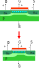
\includegraphics[width=4cm]{short-channel}
  
	\end{column}
 
\end{columns}

\end{frame}


\begin{frame}
\frametitle{Perforación del Canal}
\begin{itemize}
	\item También ocurre en canales largos a altas tensiones
	\item En canales cortos, la tensión a la que ocurre se reduce
	\item El campo entre drenador y fuente es tan intenso que la compuerta pierde el control del canal
\end{itemize}

$\Rightarrow$ Zona de agotamiento en D alcanza a tocar zona de agotamiento en S

$\Rightarrow$ El transistor no puede apagarse

$\Rightarrow$ Corriente de gran magnitud entre D y S

\centering

\includegraphics[width=7cm]{channel-perf}
\end{frame}


\begin{frame}
\frametitle{Degradación por Portadores Calientes}
\begin{itemize}
	\item Modelo del electrón afortunado (Schockley)
\end{itemize}

\begin{columns}

	\begin{column}{0.5\textwidth}
 
		\centering
		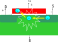
\includegraphics[width=6.5cm]{hot-carriers}
  
	\end{column}
 
	\begin{column}{0.5\textwidth}
 
		\begin{itemize}
			\item Electrón acelerado por campo eléctrico entre D y S (calentado)
			\item Electrón redireccionado hacia compuerta por colisión, inyectado en óxido
		\end{itemize}
  
	\end{column}
 
\end{columns}

Efectos: 

\begin{itemize}
	\item degradación de transconductancia
	\item cambio en voltaje de umbral (aumenta para injección de electrones en NMOS)
	\item degradación de óxido y eventualmente ruptura del mismo
\end{itemize}
\end{frame}


\begin{frame}
\frametitle{Fuga de Compuerta}
\begin{itemize}
	\item Óxido se escala para mantener el control de la compuerta sobre el canal
	\item Escalamiento de óxido aumenta la corriente de fuga de compuerta
	\begin{itemize}
		\item Efecto de tunneling cuántico (quantum mechanical tunneling)
		\item Inyección de portadores de carga
	\end{itemize}
\end{itemize}

$\Rightarrow$ Aumenta potencia de stand-by

$\Rightarrow$ Óxido no puede escalarse a tox $<$ 1 nm

\centering
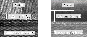
\includegraphics[width=11cm]{fuga-compuerta}
\end{frame}


\begin{frame}
\frametitle{Electromigración}

\begin{columns}

	\begin{column}{0.4\textwidth}
 
		\centering
		\includegraphics[width=3.5cm]{migration1}
		
		\vspace{5mm}
		\includegraphics[width=3.5cm]{migration2}
  
	\end{column}
 
	\begin{column}{0.6\textwidth}
 
		Desplazamiento gradual de los átomos metálicos de un conductor como resultado de la corriente fluyendo en dicho conductor
		
		\centering
		\vspace{3mm}
		\includegraphics[width=6cm]{migration3}
		
		\vspace{3mm}
		Resultado de la transferencia de momentum de los electrones a los iones metálicos que forman la red cristalina del material de interconexión
  
	\end{column}
 
\end{columns}

\end{frame}


\begin{frame}
\frametitle{El Transistor MOSFET Moderno}
\begin{itemize}
	\item Three gate: Mejor control del canal
	\item Dieléctrico: HfO\textsubscript{2}
	\item Gate: Metal (TiN para NMOS, aleación TiNAl para PMOs), con capa de baja resistencia para contacto
	\item Canal: SiGe (strain engineering), para aumentar movilidad
\end{itemize}

\centering
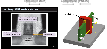
\includegraphics[width=10cm]{finFET}
\end{frame}


\begin{frame}
\frametitle{¿Qué nos espera?}

\begin{itemize}
	\item 17 Setiembre 2007: Chip de demostración con tecnología de 32nm con lógica y SRAM ya fue fabricado (1900 millones de transistores). El doble de CACHE por la misma área (2x).
	\item 2009: Proyectada producción y entrega de microprocesadores con tecnología de 32 nm (Intel)
\end{itemize}


\centering
\includegraphics[width=9cm]{intel32nm}
\end{frame}


\begin{frame}
\frametitle{¿Qué nos espera?}
\centering
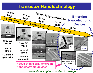
\includegraphics[width=9cm]{nanotech}
\end{frame}


\begin{frame}
\frametitle{ITRS: International Technology Roadmap of Semiconductors}

\begin{columns}

	\begin{column}{0.6\textwidth}
 
		\begin{itemize}
			\item International Technology Roadmap of Semiconductors
			\item Patrocinado por las cinco regiones líderes en manufactura de semiconductores en el mundo
			\item Resume avances de la industria microelectrónica, analiza y predice tendencias en microelectrónica
			\item Diagnostica problemas actuales para mantener el escalamiento
			\item Según ITRS, tecnología MOSFET puede llegar a alcanzar el año 2020
			\item Analiza tecnologías emergentes
		\end{itemize}
  
	\end{column}
 
	\begin{column}{0.4\textwidth}
 
		\centering \includegraphics[width=6cm]{itrs}
		
		\url{http://www.itrs2.net/}
  
	\end{column}
 
\end{columns}

\end{frame}


\begin{frame}
\frametitle{Sección Transversal de Proceso CMOS de Dos Tinas}
\centering 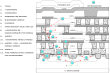
\includegraphics[width=0.8\textwidth]{CMOS-process}
\end{frame}


\begin{frame}
\frametitle{Sección Transversal de un Procesador AMD}
\centering 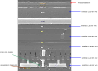
\includegraphics[width=0.7\textwidth]{AMD}
\end{frame}


\begin{frame}
\frametitle{Sección Transversal de un Circuito CMOS}
\centering 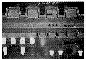
\includegraphics[width=0.7\textwidth]{CMOS-transv}
\end{frame}


\begin{frame}
\frametitle{Ejemplo de Niveles de Interconexión}
\centering 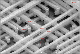
\includegraphics[width=0.7\textwidth]{CMOS-interconnect}

También llamados niveles de metalización
\end{frame}


\section{Referencias}
\begin{frame}{Lecturas recomendadas}

\begin{itemize}
    \item Moore
    \item Dennard
\end{itemize}

\end{frame}

\end{document}
